\subsection{Run-by-Run Jet QA}
The run-by-run QA of reconstructed jets in this study is assessed by analyzing the average number of jets with $p_{T} > 5$ GeV and $|\eta| < 0.7$ per event and the average jet energy per event. 
The event selections outlined in Section \ref{sec:ueinpp_selection} are implemented before analyzing these QA plots.
Figures~\ref{fig:avgNjet} and \ref{fig:avgEjet} show the distributions of the average number of jets per event and the average energy of jets per event with the above requirements.
On average, 2.1 jets are reconstructed per event and the average jet energy is approximately 15.5~GeV. 
Additionally, the number of jets per event and average jet energy is fairly consistent run-by-run across the Run 2024 p+p data taking period. 

\begin{figure}
    \centering
    \begin{subfigure}[t]{0.48\textwidth}
        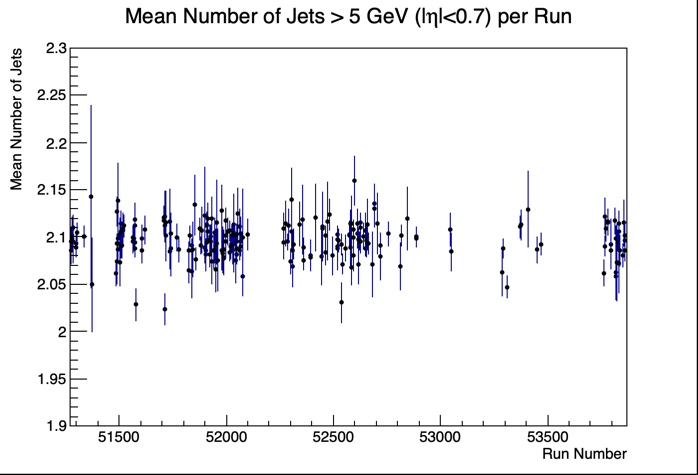
\includegraphics[width=\linewidth, trim=10 10 10 0, clip]{ueinpp/Figures/QA_Study/avg_njet_case7.png}
        \caption{Average number of jets with $p_{T} > 5$ GeV and $|\eta| < 0.7$ per event}\label{fig:avgNjet}
    \end{subfigure}
    \hfill
    \begin{subfigure}[t]{0.48\textwidth}
        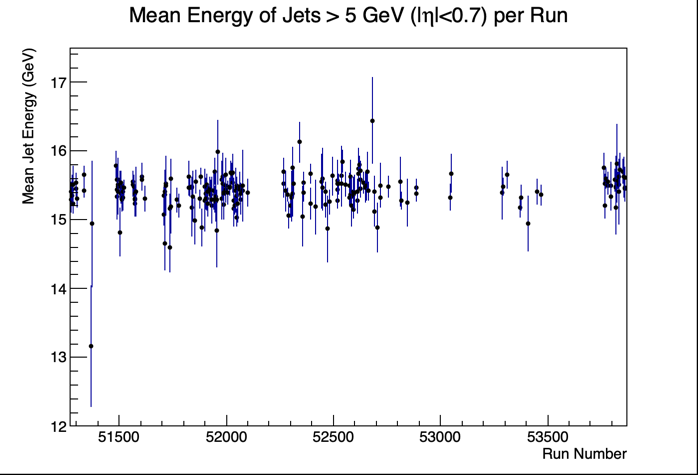
\includegraphics[width=\linewidth, trim=10 10 10 0, clip]{ueinpp/Figures/QA_Study/avg_ejet_case7.png}
        \caption{Average energy of jets $p_{T} > 5$ GeV and $|\eta| < 0.7$ per event}\label{fig:avgEjet}
    \end{subfigure}
    \caption{(a) Average number of jets per event and (b) average jet energy per event for reconstruction-level jets with $p_{T} > 5$ GeV and $|\eta| < 0.7$ shown run-by-run across the Run 2024 p+p data taking period}
    \label{fig:qa_jet_summary}
\end{figure}

\subsection{Run-by-Run Calorimeter Tower and Cluster QA}

To evaluate the stability and quality of the calorimeter response during data-taking, a run-by-run QA study on calorimeter $E_{T}$ was conducted. 
The same selection criteria as outlined in Section \ref{sec:ueinpp_selection} and applied in the jet QA study are applied here for the calorimeter tower studies.
The analysis focuses on the reconstructed-level average total transverse energy per event in the three standard jet event regions: towards, transverse, and away. 
This study is performed using calorimeter towers, EMCal clusters, and topoclusters to assess the stability of these reconstruction methods with respect to noise variations over the course of Run 2024 p+p data-taking.

\subsubsection{Average Total Transverse Energy from Calorimeter Towers}

The average total transverse energy from calorimeter towers, defined as $\Sigma E_{T} = \Sigma_i E_{T,i}^{tower}$, is evaluated separately for each calorimeter layer in the three jet event regions: towards, transverse, and away.
The average transverse energy from each layer, EMCal, IHCal, and OHCal, is shown in Figure~\ref{fig:calo_tower_et_regions}.

In the transverse region, the EMCal average transverse energy is approximately 2~GeV. This value is higher than that obtained using topoclusters (Figure~\ref{fig:avg_et_topo_case4}), but significantly lower than that from EMCal clusters (Figure~\ref{fig:avg_et_cluster_case4}). A modest run dependence of approximately 15\% is observed in the EMCal transverse region, which is consistent with increased radiation damage and the associated rise in SiPM noise over the course of the Run.

In comparison, the IHCal and OHCal transverse region average transverse energies are approximately 0.2~GeV and 0.5~GeV, respectively, both substantially lower than the EMCal contribution. These subsystems also experience less radiation damage and correspondingly smaller noise variations, resulting in improved stability over the course of the Run.

However, the combined average total transverse energy from all three calorimeter layers would exhibit a noticeable run dependence as a result of the EMCal result run dependence. This indicates that calorimeter towers are not a fully noise-insensitive reconstruction method for the average transverse energy.

\begin{figure}
    \centering
    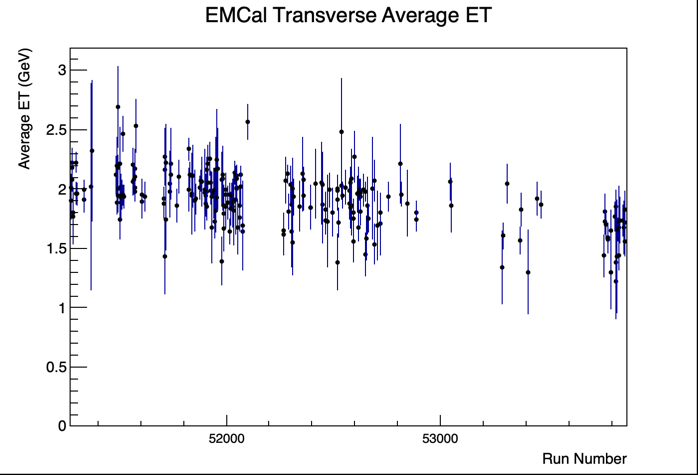
\includegraphics[width=0.48\linewidth, trim=10 10 10 0, clip]{ueinpp/Figures/QA_Study/avg_et_emcal_transverse_case5.png}
    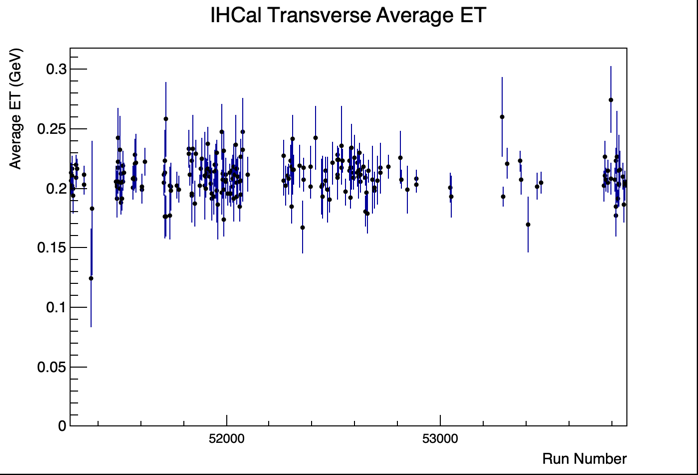
\includegraphics[width=0.48\linewidth, trim=10 10 10 0, clip]{ueinpp/Figures/QA_Study/avg_et_ihcal_transverse_case5.png}
    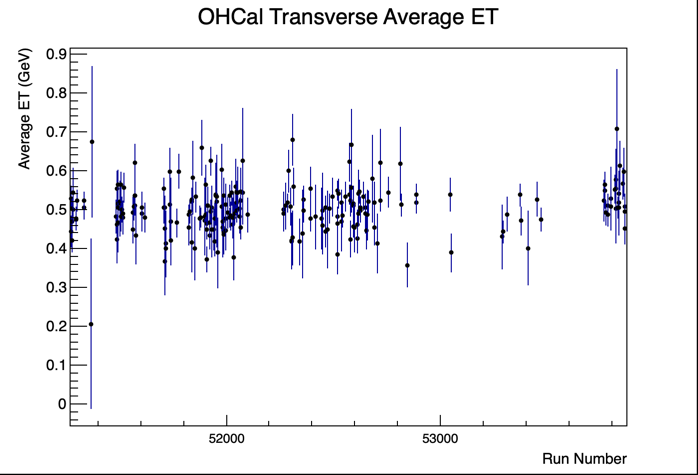
\includegraphics[width=0.48\linewidth, trim=10 10 10 0, clip]{ueinpp/Figures/QA_Study/avg_et_ohcal_transverse_case5.png}
    \caption{Average total transverse energy in EMCal (top left), IHCal (top right) and OHCal (bottom) in the transverse region shown run-by-run across the Run 2024 p+p data taking period.}
    \label{fig:calo_tower_et_regions}
\end{figure}

\subsubsection{Average Total Transverse Energy from Topoclusters}
The average transverse energy per event reconstructed using topoclusters, defined as $\Sigma E_{T} = \Sigma_i E_{T,i}^{topo}$, is evaluated as a function of run number in the transverse region. 
The average transverse energy is approximately 1.4~GeV and remains stable across the run range, indicating good performance of the topocluster-based reconstruction across the run range even with changes in run conditions, like the overall level of calorimeter noise.
In contrast to the calorimeter tower-based result, which exhibits a noticeable run dependence, the topocluster-based measurement with noise threshold optimized for the Run 2024 p+p dataset shows significantly improved stability, suggesting reduced sensitivity to variations in calorimeter noise over the course of the run.

\begin{figure}
    \centering
    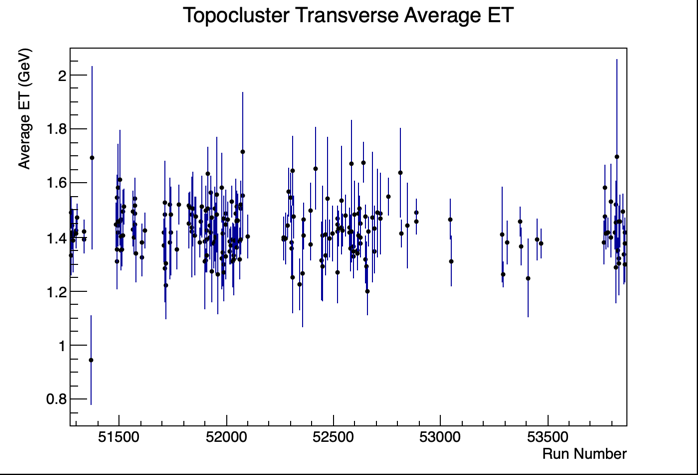
\includegraphics[width=0.6\linewidth, trim=10 10 10 0, clip]{ueinpp/Figures/QA_Study/avg_et_topo_transverse_case4.png}
    \caption{Average total transverse energy from topoclusters versus run number for transverse region shown run-by-run across the Run 2024 p+p data taking period.}
    \label{fig:avg_et_topo_case4}
\end{figure}

\subsubsection{Average Total Transverse Energy from EMCal Clusters}

To further evaluate the energy deposition patterns using a different reconstruction approach, the average transverse energy per event, defined as $\Sigma E_{T} = \Sigma_i E_{T,i}^{EMCal \: clus}$, was also studied using EMCal clusters~\cite{EMCal_calib_internal_note}. 
Here there are two obvious trends: the average transverse energy all three regions is much higher than the same observable reconstructed using just EMCal towers (see Fig~\ref{fig:calo_tower_et_regions}) and the the average transverse energy all three regions grows considerably over the course of the data-taking period. 
The EMCal clusters are highly noise dominated since they do not have a seeding requirement in the same way as the topoclusters and the tower threshold for the EMCal cluster reconstruction is set right in the middle of the noise spectrum at a value of 70 MeV. Therefore, the average total transverse region \ET{} extracted from EMCal clusters is 5 times that extracted from EMCal towers (Fig~\ref{fig:calo_tower_et_regions}) and changes 35\% over the course of the Run.
The EMCal clusters are not a good noise-insensitive reconstruction method for the average transverse energy. 

\begin{figure}
    \centering
    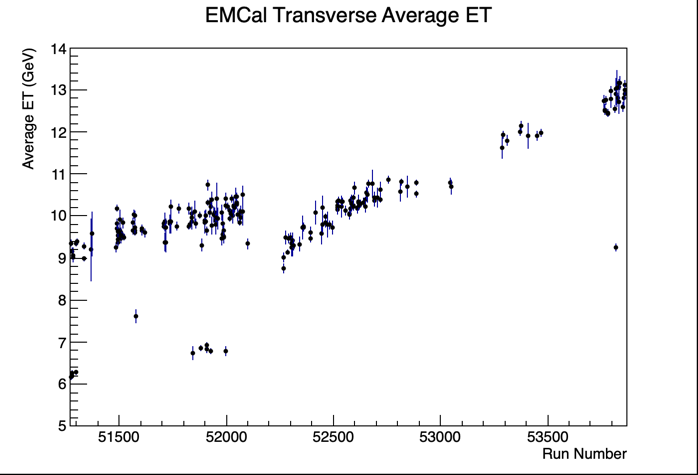
\includegraphics[width=0.6\linewidth, trim=10 10 10 0, clip]{ueinpp/Figures/QA_Study/avg_et_cluster_transverse_case4.png}
    \caption{Average total transverse energy from EMCal clusters versus run number in the transverse region shown run-by-run across the Run 2024 p+p data taking period.}
    \label{fig:avg_et_cluster_case4}
\end{figure}